\documentclass[preprint]{aastex}
\usepackage{amsmath,amssymb}
\usepackage{mathrsfs}
\usepackage{graphicx}
\newcommand{\mli}[1]{\mathit{#1}}
%\usepackage{epstopdf}


\bibliographystyle{plain}


\begin{document}

\title{Type Ia Supernova Model}
\author{Alex Kim}

\section{Model}
Supernova cosmology analysis is based on the Hubble diagram: measurements of
redshift $z$ and distance modulus $\mu$.  The inferred Hubble diagram
can be expressed as the pdf of the true underlying
quantities given these measurements 
\begin{equation}
P(\vec{\mu},\vec{z}| \vec{\hat{\mu}}, \vec{\hat{z}}, \vec{\hat{D}}=1, \vec{\hat{T}}=\text{SN~Ia}),
\end{equation}
where $\hat{D}=1$ and $\hat{T}=\text{SN~Ia}$ indicate that the objects are discovered and typed
as SNe~Ia.  
The caret labels measurements and quantities derived
from measurements.  This Hubble diagram can then be used to infer parameters
of cosmological and dark energy models.

A model of the experiment is necessary to interpret the data, as in the
calculation of the likelihood function $P(\vec{\hat{\mu}}, \vec{\hat{z}}, \vec{\hat{D}}=1, \vec{\hat{T}}=\text{SN~Ia}|\vec{\mu},\vec{z})$.
A sketch of a such a model is shown in the Probabilistic Graphical Model
shown in Figure~\ref{pgm:fig}.

\begin{figure}[htbp] %  figure placement: here, top, bottom, or page
   \centering
   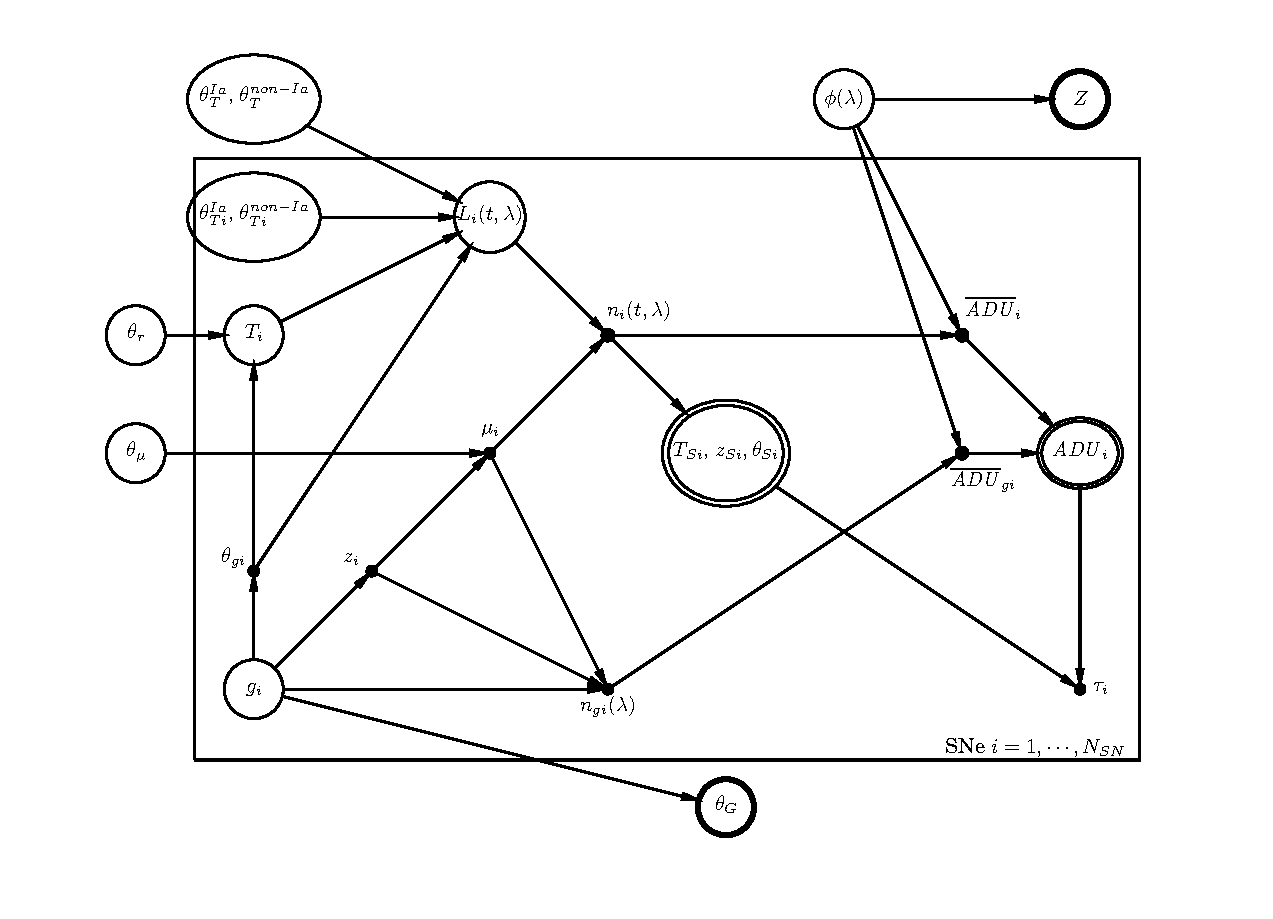
\includegraphics[width=7in]{/Users/akim/project/abc/results/hdpgm.eps} 
   \caption{Probabilistic Graphical Model for the SN~Ia analysis.
   The bottom right corner containing the connection between observed light curves
   $\hat{f}$, transient spectral information $\hat{z}_S$, $\hat{\theta}_S$, and
   host information $\hat{z}_H$, $\hat{\theta}_H$ with the determined type, redshift, and distance
   modulus $\hat{\mathit{Type}}$, $\hat{z}$, and $\hat{\mu}$ is the purview of
   the traditional light-curve and Hubble diagram fitters.
   \label{pgm:fig}}
\end{figure}

\subsection{Forward Model}
I first walk through the PGM as a forward process.  This is useful for understanding
how the model would be simulated.

There is a set of redshifts
at which a transients explode $\vec{z}$ and for each (cosmological) redshift there is a corresponding distance
modulus $\vec{\mu}$; these $z$-$\mu$ pairs are the fundamental parameters that
specify the Hubble diagram.

Given that there is a transient at redshift $z$, it has a probability of being a particular
Type associated with a Host. 
The Host is anything that projects onto the line of sight of the transient and so contributes
to measurement noise.   For our purposes, the Type and Host include information on the
sources and line-of-sight effects that can be encapsulated as an effective SED. 
This SED and distance modulus determine the photon flux incident above the Earth's
atmosphere, $n$ and $n_g$.

The experiment has an optical chain summarized by the transmission functions $T(\lambda)$, which determine the expected counts of the transient and galaxy, $\mathit{ADU}$ and
$\mathit{ADU}_g$.  
The realized observed counts determine whether the transient
is discovered $\hat{D}$, and the 
calibration $\hat{Z}$ of the transmission functions set the
measured flux-calibrated light curves $\hat{f}$.  

Spectra $\hat{\mathit{Spec.}}$ may be obtained for active candidates, from which typing, redshift and spectral parameters $\hat{z}_S$, $\hat{\theta}_S$ are derived.
From the detected galaxies Gals.\ a host is associate with the transient, the measured
host redshift and parameters are $\hat{z}_{H}$, $\hat{\theta}_H$.

Given the transient light curves, spectra, and host-galaxy measurements, the transient
type $\hat{\mathit{Type}}$, redshift $\hat{z}$, and distance modulus $\hat{\mu}$ are
determined.  Depending on what information is available, this is done by some combination
of a light-curve fitter, classifier, and empirical SN~Ia modeler; in this note this black box
is referred to as a Fitter.

\subsection{Backward Model}
 
I now systematically
examine the model going backwards, from the observables to the fundamental parameters.
This is useful for understanding dependencies in constructing the likelihood.

\begin{description}
\item[$\hat{D}$] Transient detection.  It depends on
the observed signal $\hat{f}$ and its noise, mostly through the signal-to-noise
$\mathit{SNR}$.
\item[$\hat{z}$] Cosmological redshift.  There is an ordering of how the redshift
is determined. If there is an unambiguous host its spectroscopic redshift $\hat{z}_H$ is
selected.  Next, the transient's spectroscopic redshift $\hat{z}_S$ is preferred.
Generally these spectroscopic redshifts have negligible uncertainties for our purposes.
When the host is ambiguous, has only a photometric redshift, and/or there is
no transient redshift,
the calibrated supernova light curve $\hat{f}$ and all other information is combined to
infer redshift.
\item[$\hat{\mathit{Type}}$] Transient classification.  Traditionally only objects
typed as SN~Ia are used in the analysis: alternatively a probability of being
SN~Ia could be used.  The soundest classification comes from a transient
spectrum $\hat{\mathit{Spec}}$.  Otherwise typing is informed by host information
$\hat{z}_H$ and $\hat{\theta}_H$, and
calibrated light curves $\hat{f}$.
\item[ $\hat{\mu}$]  Distance modulus.  This is typically done with a light-curve
analysis using $\hat{f}$, $\hat{z}_S$ or
$\hat{z}_H$, and transient spectral features $\hat{\theta}_S$ and host
properties $\hat{\theta}_H$.
\end{description}

Generically the typing, redshift, and distance modulus are obtained
using a Fitter, with the details depending on the available information.
A calibration of the empirical SN~Ia absolute magnitude model is fit in this step.
Therefore $\hat{z}$, $\hat{\mathit{Type}}$
and $\hat{\mu}$ may be correlated, and correlations between transients are expected.

\begin{description}
\item[$\hat{z}_H$, $\hat{\theta}_H$] Host galaxy redshift and properties from spectroscopic
and photometric data, based on association
of the host from the pool of detected galaxies Gals.
\item[Gals] Detected galaxies from which a host is associated with a transient.
\item[$\hat{z}_S$, $\hat{\theta}_S$] Transient redshift and properties from
spectroscopic data $\hat{\mathit{Spec.}}$
\item[ $\hat{\mathit{Spec.}}$] Spectrum of the transient. I skip the details of the actual measurement  make a direct association
with the fluxes of the transient and underlying galaxy $n$, $n_g$.
\item[$\hat{f}$] Measured light curves.  Depends on the expected counts of
the transient and background $\mathit{ADU}$, $\mathit{ADU}_g$
(as a contributor to noise), and the photometric zeropoints $\hat{Z}$.
\item[$\hat{\mathit{ADU}}$, $\hat{\mathit{ADU}_g}$]  Expected counts
of the transient and background galaxy respectively.  Depends
on the incident fluxes $n$, $n_g$ and the instrumental
transmission $T(\lambda)$.
\item[$\hat{Z}$] Calibration zeropoints.  Depends on the calibration process
and the underlying transmission functions $T(\lambda)$.  This may be a zeropoint
but most probably will be calibratied transmission functions.
\item[$T(\lambda)$] DES transmission functions.
\item[$n$, $n_g$] The incident fluxes at Earth of the transient and background
galaxy.  Depends on  $z$ and $\mu$, and the SEDs of the Type and Hiost.
\item[Type/Host]  The type of transient and projected galaxies (referred to as host),
used to the specify the
underlying SED.  The realization depends on the redshift $z$.
\item[$\vec{\mu}$, $\vec{z}$]  The true distance moduli and cosmological redshifts under
consideration.  Each redshift has a unique distance modulus.
\end{description}

\section{Comments on Parts of the Model}

\subsection{Type}
The model allows for transients of all types to be detected
and potentially classified as SN~Ia. 
The full population of potential interlopers and their rates, $P(\text{Type} | z)$,
is poorly constrained.
I therefore propose that the model be constrained to SNe~Ia only,
and have the experiment measure
$P(non-Ia |  \hat{\mathit{Type}}=\text{SN~Ia})$,
$\left. \langle \hat{\mu}-\mu(z)\rangle \right|_{non-Ia}$ and its uncertainty.
This would be added as a correction to the Hubble diagram under the assumption
that all objects are SNe~Ia.

\subsection{The Fitter}
The model contains the term
\begin{align}
\begin{split}
P(\hat{\mu},\hat{z}, \hat{D}=1, \hat{\mathit{Type}}=\text{SN~Ia}|X) & =  P(\hat{D=1}|X) P(\hat{\mu},\hat{z},\hat{\mathit{Type}}=\text{SN~Ia}|X)\\
&=  P(\hat{D=1}|\hat{f}) P(\hat{\mu},\hat{z}, \hat{\mathit{Type}}=\text{SN~Ia}|X)\\
\end{split}
\label{fitter:eqn}
\end{align}
where $X=\{\hat{f}, \hat{\mathit{Spec.}}, \hat{z}_S, \hat{\theta}_S, \hat{z}_H, \hat{\theta}_H\}$
represents relevant measurements.  The first term on the right side of Eqn.~\ref{fitter:eqn}
is the detection efficiency.  The second term is what I have generically called the
Fitter.

Traditional supernova cosmology analysis is covered by the arrows that lead to
the measured type, redshift, and distance modulus.  Within this larger
context, probably the supernova absolute magnitudes should be calibrated relative
to a model that does not depend on the cosmological parameters.

Need to calibrate $P(x|y,\hat{T=\text{SN~Ia}})$.

\end{document}

